\subsection{Autoencoder}

The autoencoder is a type of network used to learn efficient encodings of unlabeled data. 

Autoencoders are split into two parts. The encoder $E_\phi$ and the decoder $D_\theta$. The relationship between these can be articulated as such: 

\begin{figure}[h]
    \centering
    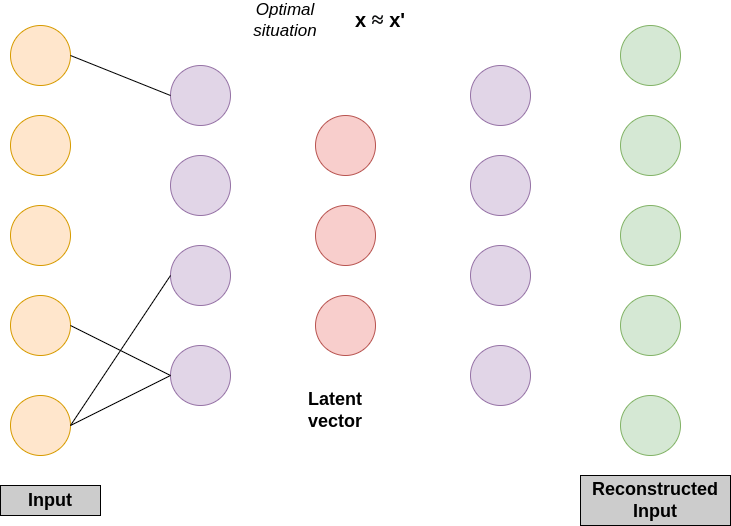
\includegraphics[scale=0.5]{figures/ae.png}
    \caption{Autoencoder Architecture Diagram}
    \label{fig:aediagram}
\end{figure}

\begin{equation}
E_\phi: X \rightarrow Z 
\end{equation}

\begin{equation}
D_\theta: Z \rightarrow X
\end{equation}

The optima for any kind of autoencoder becomes that of lossless encoding, which can further be described as such:

\begin{equation}
    X = D_\theta(E_\phi(X))
\end{equation}

When a auto encoder is trained to max effiency, we can in some cases remove the decoder part. Since the goal in the beginning was to map data to a lower-dimensional latent space, which has been increased. If ones goal is feature extraction, the decoder is not needed any more. Additionally, by removing the decoder, the overall complexity and size of the model $M$ decreases.


Typical usecases for autoencoders are signal analysis, anomaly detection, reconstructing images and so on. 
One of the more well known usages for autoencoders

\subsubsection{Loss functions}

\textbf{\acrfull{mse}}

The \acrshort{mse} loss function, also referred to as L1 loss, is one of the most well known loss functions. It punishes bigger differences by squaring the difference between two elements in the prior and the posterior.

\begin{equation}
    MSE = \dfrac{1}{n}  \sum_{i=1}^{n}(x_i-\hat{x}_i)^2
\end{equation}

\textbf{\acrfull{mae}}

The \acrshort{mae} loss function, also referred to as L2 loss, is quite similar to the L1 loss. The difference is that the \acrshort{mae} function will only return the absolute value of the difference between two distributions, thus not caring about the difference itself.

\begin{equation}
    MAE = \dfrac{1}{n}  \sum_{i=1}^{n}|x_i-\hat{x}_i|
\end{equation}

\textbf{Hinge Loss}

\begin{equation}
    L = \max(0, 1 - x \cdot \hat{x}))
\end{equation}

\textbf{Log Loss, VAE}

The log loss, also known as Binary Cross Entropy loss

\begin{equation}
L(x, \hat{x}) = - \frac{1}{N} \sum_{i=1}^{N} \left( x_i \log(\hat{x}_i) + (1 - x_i) \log(1 - \hat{x}_i) \right)
\end{equation}


\textbf{Activation Functions}
\begin{equation}
    ReLU(z) = max(0, z)
\end{equation}

\subsubsection{Variational Autoencoder (\acrshort{vae})}

Similar to the regular autoencoder, a \acrfull{vae} also aims to map input over to a feature representation. The diffre. Broadly speaking, the difference between a \acrshort{ae} and a \acrshort{vae} is that a AE maps input to points, where as VAEs map over to a distribution in the latent space. The encoder $E$ outputs to vectors. 

Thus, the \acrlong{vae} can be seemed as a generative model.


\begin{figure}[h]
    \centering
    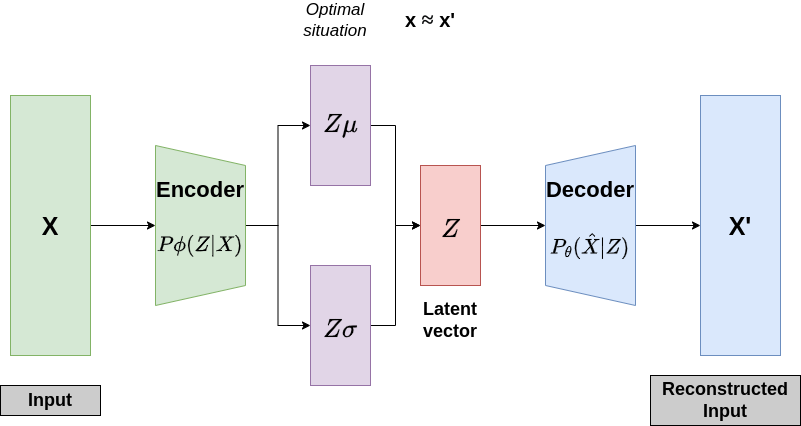
\includegraphics[scale=0.5]{figures/vae.png}
    \caption{Variational Autoencoder Architecture Diagram}
    \label{fig:vaediagram}
\end{figure}


VAEs can be trained by backpropagation due to something known as the \textit{reparametrization trick}. We need this because since VAEs maps to a stochastic variable, abckpropagation would else not be feasible.

\begin{align*}
\text{Given:} & \quad \text{Encoder LSTM outputs: } h \\
& \quad \text{Mean vector: } \mu \\
& \quad \text{Log variance vector: } \log(\sigma^2) \\
\text{Sample:} & \quad \epsilon \sim \mathcal{N}(0, 1) \\
\text{Reparameterization:} & \quad z = \mu + \sigma \odot \epsilon \\
\text{Decoder Input:} & \quad z \quad \text{(sampled latent vector)} \\
\text{Training Objective:} & \quad \text{Minimize reconstruction error} \\
& \quad \text{and KL divergence between } q(z|x) \text{ and } p(z) \\
\text{Loss Function:} & \quad \mathcal{L} = \text{reconstruction\_loss} + \text{KL\_divergence}
\end{align*}


\textbf{KEYS TO GETTING A GOOD VARIATIONAL AUTO ENCODER}

\begin{itemize}
    \item Pick the righ size for the latent space
    \item Learning rate scheduler  and hyperparam tuning 
    \item BETA COEFFICIENT
\end{itemize}

An effort has been made into trying to improve autoencoders for anomaly detection \cite{tan2023improving}

THIS ONE IS HIGHLY RELEVANT AND HAS MANY METRICS \cite{s23021009}